
\documentclass[preprint,12pt]{elsarticle}

\usepackage[spanish]{babel}
\usepackage{amssymb}
\usepackage{graphicx}
\usepackage{lineno}
\usepackage[utf8]{inputenc}
\usepackage{url}
\usepackage{natbib} 
\usepackage{amsmath} 
\usepackage{amssymb} 

\begin{document}
	
	\begin{frontmatter} 

		\title{\huge Gestores de BD NoSQL}
		
		\author{Estrella Palacios, Katherine Lizbeth      (2016056193))}
		\author{Andia Zeballos,Alonso André           	(2016054945))}
		\author{Porlles Carrillo, Diego Armando	         	(2015050948))}  
		\author{Mamani Mamani, Pedro Luis                 (2010038808))} 
		\address{Escuela Profesional de Ingeniería de Sistemas}
		\address{Universidad Privada de Tacna}
		\address{Tacna, Perú}
		
%% ABSTRACT --------------------------------------------------------------------------------------------------------------------

		\begin{abstract}
		
NoSQL databases have experienced a significant increase in their application in recent times. The great flexibility they offer and the possibilities they offer from the point of view of optimization in their designs according to the problem to be solved make them an attractive variant to consider for developers of information management applications. \\ \\ This article will address the topic of graph-oriented databases (BDOG), also mentioned as an example NEO4J.

		\end{abstract}

%% ----------------------------------------------------------------------------------------------------------------------------------

	\end{frontmatter}

%% RESUMEN ---------------------------------------------------------------------------------------------------------------------

\section{Resumen}

Las bases de datos NoSQL han experimentado un importante incremento en su aplicación en los últimos tiempos. La gran flexibilidad que ofrecen y las posibilidades que brindan desde el punto de vista de la optimización en sus diseños de acuerdo al problema a resolver las convierten en una atractiva variante a tener en cuenta para los desarrolladores de aplicaciones de gestión de información.\\ \\  En el presente artículo se abordará el tema de bases de datos orientadas a grafos (BDOG), también se mencionará como ejemplo NEO4J.

%% ----------------------------------------------------------------------------------------------------------------------------------


%% INTRODUCION ----------------------------------------------------------------------------------------------------------------

\section{Introducción} 

Las bases de datos relacionales tienen una amplia aceptación en el mundo del desarrollo de software y han demostrado su efectividad en los distintos contextos en los que se ha aplicado a la hora de realizar el almacenamiento de información; sin embargo, los tiempos han cambiado y la información ha evolucionado a tal punto que los sistemas de información se tienen que encontrar con la manipulación de grandes cantidades de datos, lo cual ha resultado difícil y se han  mplementado otras estrategias para manejar la información.

Con la alta demanda que se requiere al momento de almacenar información y la gran capacidad que se necesita en las aplicaciones informáticas cuando se realizan consultas sobre ellas, ha generado la búsqueda de nuevas herramientas tecnológicas que ayuden a tener una mejor gestión de los datos. Recordemos que en muchas ocasiones los datos necesitan ser analizados e interpretados para convertirlos en información útil y provechosa, tal situación ha propiciado una creciente necesidad por técnicas/herramientas computacionales que nos ayuden en estas tareas. Por lo tanto, si pudiéramos representar los datos y las relaciones entre objetos como un solo conjunto de datos, podríamos generar patrones de conocimiento que describan nuestro conjunto de datos conteniendo estos elementos de manera conjunta. Para tal efecto se presentan las bases de datos en grafos que son lo suficientemente flexibles y poderosas para representar estos elementos. Se utiliza la estructura de control “grafos”.



%% ----------------------------------------------------------------------------------------------------------------------------------


%% MARCO TEÓRICO ------------------------------------------------------------------------------------------------------------

\section{Marco Teórico}

%% PRIMERA SUBSECCION 

\subsection {\textbf{Base de Datos No Relacional}}

Una base de datos no relacional (NoSQL) es aquella base de datos que:

\begin{itemize}
	\item No requiere de estructuras de datos fijas como tablas
	\item No garantiza completamente las características ACID
	\item Escala muy bien horizontalmente.
\end{itemize}

Se utilizan en entornos distribuidos que han de estar siempre disponibles y operativos y que gestionan un importante volumen de datos.


\subsubsection{\textbf{Base de datos orientada a Grafos (BDOG)}}

Una base de datos orientada a grafos es aquella que permite almacenar la información como nodos de un grafo y sus respectivas relaciones con otros nodos, permitiendo así aplicar la teoría de grafos para recorrer la base de datos; son muy útiles para guardar información en modelos con muchas relaciones como redes y conexiones sociales. 

Cada nodo consta de un grado que indica el número de aristas que tiene, a su vez un grafo puede ser dirigido o no dirigido, dependiendo de si las aristas tienen nodos origen y nodos destino. El uso de este tipo de bases de datos depende altamente de la lógica de negocio donde se encuentre involucrada la información a almacenar, ya que no puede aplicar en todos los escenarios, o tal vez no se podría aprovechar su potencial en unos u otros contextos. 

Un grafo estará compuesto por dos elementos: los nodos (vértices) y las relaciones (aristas). Un nodo representa una entidad, en el que almacenaremos piezas de datos o atributos de tipo clave-valor, mientras que las relaciones representan cómo se conectan y se asocian dos nodos.

\begin{figure}[htb]
	\begin{center}
		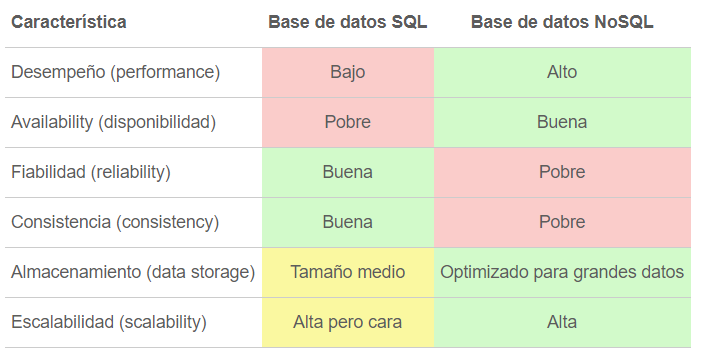
\includegraphics[width=9cm]{./IMAGENES/basededatos_3} 
		\caption{Tabla comparativa entre Base de Datos SQL y NoSQL}
	\end{center}
\end{figure}

Las clasificamos como NoSQL por las siguientes características:
\begin{itemize}
     \item No utilizan un modelo relacional 
     \item Carece de un esquema fijo, podemos tener nodos con diferente número de atributos.  
     \item Mantienen la disponibilidad y acceso de la información
     \item Son buenas en modelos en cluster
\end{itemize}

Sus características principales son:
\begin{itemize}
 \item Son multidimensionales, pueden almacenar atributos de diverso tamaño en los nodos
 \item Las relaciones pueden almacenar atributos
 \item Las relaciones pueden ser sin dirección, unidireccionales y bidireccionales lo que puede convertir la representación a grafos dirigidos, muy útiles en el cálculo de caminos.
 \item Tienen alto rendimiento en la búsqueda de resultados y sobre todo en la búsqueda de caminos.
\end{itemize}


\subsubsection{\textbf{NEO4J}}
Es una base de datos orientada a grafos que se compone de dos elementos fundamentales:
\begin{itemize}
 \item Nodos, que representan entidades con un concepto de identidad único. 
 \item Relaciones, que representan conexiones o interacciones entre los diferentes nodos.
\end{itemize}
Tanto los nodos como las relaciones pueden contener propiedades, que son equivalentes a las columnas de las tablas en el modelo relacional. 
\\ \\ La siguiente imagen muestra un ejemplo de base de datos en Neo4j:

\begin{figure}[htb]
	\begin{center}
		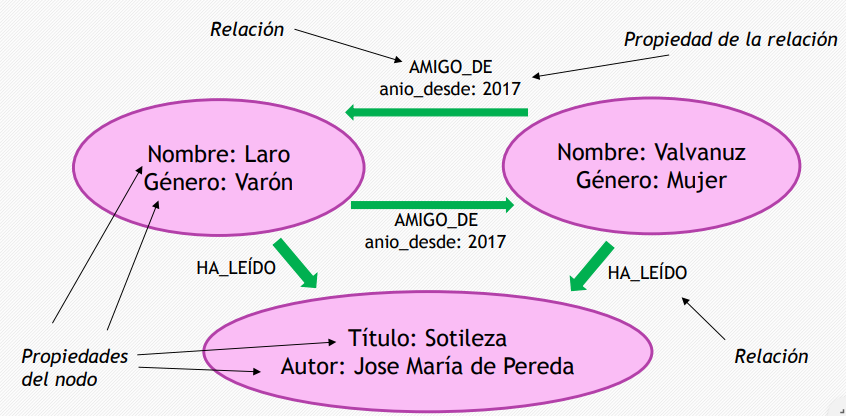
\includegraphics[width=9.5cm]{./IMAGENES/ejemplo_neo4j} 
		\caption{Ejemplo de Base de Datos en Neo4j}
	\end{center}
\end{figure}

Los nodos puede tener etiquetas (ninguna o varias), que se utilizan para agruparlos. En el ejemplo anterior, podríamos definir dos etiquetas: una llamada “personas” (en naranja), que asignaríamos a Laro y Valvanuz, y otra llamada “libros” (en morado), que asignaríamos al nodo restante:

\begin{figure}[htb]
	\begin{center}
		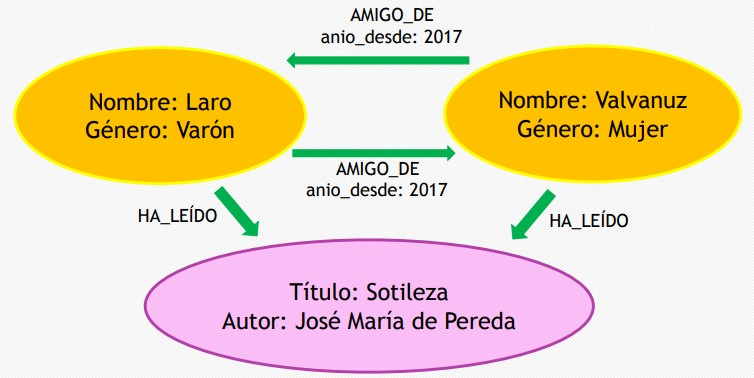
\includegraphics[width=10.5cm]{./IMAGENES/NEO4J_ejemplo} 
		\caption{Ejemplo de Base de Datos en Neo4j - Etiquetas}
	\end{center}
\end{figure}

\textbf{Lenguaje de consulta y manipulación de datos: Cypher\\}

Cypher es el lenguaje desarrollado por Neo4j para la creación de bases de datos así como para realizar operaciones de inserción, modificado, borrado y consulta de los datos.
\begin{itemize}
 \item Es un lenguaje declarativo, inspirado en SQL.
 \item Orientado a la descripción de patrones en grafos.\\
\end{itemize}

En Cypher, los tipos de datos se dividen en dos grupos: 


\begin{itemize}
 \item Básicos: Booleano, Integer, Float, String, List,  Map
 \item De estructura: Node, Relationship, Path
\end{itemize}



%% ----------------------------------------------------------------------------------------------------------------------------------
 
\newpage

%% ANÁLISIS ( APLICACIÓN ) ---------------------------------------------------------------------------------------------------

\section{Análisis}

\subsection{\textbf{Comparación modelo relacional}}
El modelo relacional es ampliamente conocido, se puede comprender como un conjunto de entidades que se relacionan con otras. En el proceso de modelamiento se trasladan a tablas, por lo que en práctica se diseñan tablas con columnas para representar a cada entidad y a cada relación, para esto el experto debe seguir procesos de normalización y otros procedimientos para representar el modelo de negocio teniendo presente los lineamientos y restricciones propias de las bases de datos relacionales.\\

Para una simple relación entre dos entidades, se debe modelar una tabla con los atributos que la identifican a cada entidad, y según sea el tipo de relación, pueden surgir una o varias tablas que representan la relación. Aunque la generación de las tablas para las relaciones es el resultado de aplicación de las reglas de normalización, constituyen un elemento para tener en cuenta en el modelamiento.\\

En el modelo de estructura de grafos se tienen dos tipos de elementos: los nodos y las relaciones, cada uno de ellos contienen sus propiedades tipo clave valor; asimismo las relaciones agregan una característica y es que pueden ser o no dirigidos. En grafos cada elemento, entiéndase nodo y relación, tiene su espacio propio y no necesariamente está limitado a representar un solo tipo de dato, pues en casos específicos, un nodo puede representar diferentes tipos de datos disponibles según el propósito con que se modelen; también un elemento o nodo que represente un tipo de dato es identificable además por las relaciones que tiene con otros nodos. La principal diferencia mcon las bases de datos relacionales es su poder de consulta y la libertad en el esquema de datos.\\


\subsection{\textbf{Fortalezas}}
El uso de las bases de datos orientadas a grafos puede tener ventajas en escenarios donde los sistemas a implementar requieran de una adaptación constante a los cambios de lógica de negocio, y en modelos donde existe una alta dependencia funcional entre las entidades involucradas en un sistema. \\

El rendimiento es una fortaleza clave para el uso de bases de datos con grafos; en comparación con el uso de bases de datos relacionales, donde su rendimiento está fuertemente ligado al tamaño de los datos y las numerosas relaciones entre las entidades, implicando que el rendimiento en las consultas esté inversamente proporcional a la totalidad de los registros y relaciones envueltas entre las entidades que satisfacen la consulta, en BDOG el rendimiento tiende a permanecer  relativamente constante, ya que las consultas se realizan iniciando un recorrido desde un segmento de datos del grafo, pasando por los distintos nodos y aristas necesarios para satisfacer la consulta, dando como resultante que el tiempo de ejecución es proporcional únicamente al tamaño del grafo que se tenga que recorrer para satisfacer la consulta, no el tamaño total del grafo.

En un sistema donde se presenten múltiples niveles de profundidad de los datos relacionados, se evidencia la rapidez de la ejecución de consultas en bases de datos orientadas a grafos. \\

\subsection{\textbf{Aplicación BDOG–Scrum}}
Pensar en una aplicación de las bases de datos orientadas a grafos diferentes a las normalmente conocidas vistas anteriormente no es una tarea fácil, primero, porque es cambiar un paradigma, un pensamiento que se ha inducido con el uso frecuente de las bases de datos relacionales desde las etapas de preparación universitaria hasta el ejercicio profesional de la ingeniería de sistemas; segundo, debido a que normalmente el proceso de definición y utilización de una base de datos se realiza basado\\

Bajo esta premisa, se propone un uso de BDOG aplicado en el elemento Scrum Board. Esta
propuesta consiste en una alternativa diferente al seguimiento de las tareas por Sprint en un marco de trabajo Scrum, dado que los datos bajo este contexto pueden evolucionar a medida que evoluciona el negocio y se encuentran altamente relacionados; se trata de almacenar los elementos que se encuentran involucrados durante el proceso de un Sprint en un proyecto Scrum como un árbol de grafos con raíz con cuatro niveles. Los niveles que se encuentran altamente relacionados en este proceso son:
\begin{itemize}
\item Proyecto: identificado por una etiqueta como el nombre del sistema o producto que se está implementando.
\item PBI: los diferentes ítems del product backlog que contienen las características funcionales a implementar del producto.
\item Sprint: identificador de cada uno de los Sprints generados para cumplir con uno o varios ítems de los product backlog.
\item Tarea: compromisos adquiridos en cada Sprint, para satisfacer una o varias características funcionales establecidas en los PBI.
\end{itemize}

\begin{figure}[htb]
	\begin{center}
		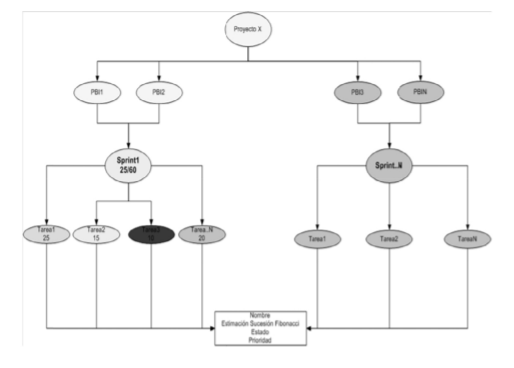
\includegraphics[width=13cm]{./IMAGENES/basededatos_4} 
	\end{center}
\end{figure}

El proyecto se comportaría como el nodo raíz del sistema, seguido por un nivel donde estarán representados los ítems del product backlog definidos
previamente para todo el proyecto, comportándos  como nodos hijos del nodo raíz. El siguiente nivel se relaciona con cada uno de los Sprints donde
se encuentran involucrados uno o varios ítems del product backlog representándolos como nodos hijos de los PBIS, por último, se encuentran las tareas
como un último nivel del árbol de grafos, las cuales se representan como nodos hijos de un elemento Sprint (Figura 3).

\subsection{\textbf{Casos de Uso}}
El uso de una BDOG es una respuesta a la dificultad de representar los diversos sistemas complejos que caracterizan al mundo actual, y a la necesidad de tener un alto performance de un sistema que se encuentre involucrado en contextos con altos volúmenes y concurrencia de datos. Actualmente, las bases de datos orientadas a grafos se están aplicando en los casos descritos a continuación. \\

\begin{itemize}
\item Redes sociales: las personas o grupos corresponden a nodos en una base de datos orientada a grafos, y las formas como interactúan dichos individuos generan las distintas relaciones de los mismos permitiendo así predecir sus comportamientos.\\

\item Recomendaciones: los algoritmos de recomendación establecen las relaciones entre individuos y los servicios a los que pueden estar sometidas las personas. Ya sea al momento de realizar una lectura de interés, la visualización de algún video, las compras que realice una persona o las diversas variedades de consumo de los individuos tienden a establecer un interés en algún tema en particular generando una conducta de la cual se pueden abstraer y almacenar múltiples relaciones para su posterior recomendación. \\

\item Geo: las distintas operaciones geoespaciales dependen de estructuras de datos específicos, las cuales se pueden representar de una forma jerárquica; dicha representación facilita los cálculos de rutas o cualquier obtención de información entre las ubicaciones en alguna red específica tales como la de carreteras, ferroviaria o espacio aéreo. Las aplicaciones geoespaciales de las bases de datos orientadas a grafos son especialmente relevantes en las áreas de  telecomunicaciones, logística, viajes, horarios y planificación de rutas. \\

\item Controles de acceso: la autorización del uso de recursos o aplicaciones por parte de los diferentes tipos de usuarios basados en sus roles en un sistema permite que dicho flujo de información pueda ser representada mediante la utilización de grafos.  \\

\end{itemize}



%% ----------------------------------------------------------------------------------------------------------------------------------


%% CONCLUSIONES ---------------------------------------------------------------------------------------------------------------

\section{Conclusiones}

\begin{itemize}

\item  Las bases de datos orientadas a grafos son una clara alternativa a las bases de datos tradicionales, sobre todo para algunas aplicaciones sociales y web que requieren elevada escalabilidad. Estas bases de datos no son idóneas para todo, de hecho en la mayoría de los casos las bases de datos relacionales deberían seguir siendo la primera opción, debido a la capacidad de hacer JOIN y ciertas garantías que son muy importantes en algunas aplicaciones. \\ 

\item Algo importante a decir es que debido al uso de las bases de datos orientadas a grafos es muy posible que las bases de datos tradicionales actuales evolucionen para incorporar capacidades NoSQL y así mejorar los motores de bases de datos obteniendo una persistencia transaccional polígota. \\ 

\item Como hemos visto a lo largo del artículo, las BDOG nos ofrecen una gran versatilidad frente a otros modelos de tipos NoSQL y las recomendamos utilizar en los casos en los que se haga un principal hincapié en las relaciones de relación entre las entidades junto con un modelo de la información datos, flexible. \\

\item Las BDOG facilitan la exploración de los datos gracias a su naturaleza de estructura de grafo, permitiendo hacer recorridos por caminos cortos del grafo sin necesidad de verificar la totalidad de caminos del árbol de grafos. Además, los algoritmos de búsqueda, descubrimiento de caminos cortos, exploración en anchura y profundidad que incluyen estas base de datos son temas que resultan muy interesantes seguir aprendiendo sobre ello.\\ 


\end{itemize}

\newpage
%% ----------------------------------------------------------------------------------------------------------------------------------

%%  REFERENCIAS BIBLIOGRÁFICAS ------------------------------------------------------------------------------------------
	
\section{Referencias}

[1] Silberschatz, A., Korth, H. and Sudarshan, S. (1996).
Data Models. ACM Computing Surveys, 28(1),
105–108 \\

[2] Penchikala, S. (2014). Data Modeling in Graph Databases: Interview with Jim Webber and Ian Robinson. Recuperado de http://www.infoq.com/articles/
data-modeling-graph-databases. \\

[3] Marín, R. (2019). Los gestores de bases de datos más usados en la actualidad. Recuperado de https://revistadigital.inesem.es/informatica-y-tics/los-gestores-de-bases-de-datos-mas-usados/ \\

[4] Pinilla, C. (2017). Bases de datos orientadas a grafos. Recuperado de https://revistas.udistrital.edu.co/index.php/tia/article/view/8769/pdf \\

[5] Velasquez, W. (2017). Algoritmo de recomendación sensible a contexto de elementos educativos reutilizables con almacenamiento Orientado a Grafos. Recuperado de http://www.rte.espol.edu.ec/index.php/tecnologica/article/view/311/359 \\

[6] Zorrilla, M. (2017). Gestores NoSQL – Neo4j. Recuperado de https://ocw.unican.es/pluginfile.php/2396/course/section/2473/NoSQL\_Tema2\_Neo4j.pdf \\
	


%% https://revistadigital.inesem.es/informatica-y-tics/los-gestores-de-bases-de-datos-mas-usados/
%% http://www.rte.espol.edu.ec/index.php/tecnologica/article/view/311/359
%% https://n9.cl/7v7f
%% https://revistas.udistrital.edu.co/index.php/tia/article/view/8769/pdf
%% https://ocw.unican.es/pluginfile.php/2396/course/section/2473/NoSQL_Tema2_Neo4j.pdf   <--- NEO4J
	
\end{document}
